
\chapter{Réalisation}
\lipsum[7-8]
\section{Difficultés rencontrées}
\subsection{Problèmes de son}
Au tout début du projet nous avons eu l'idée d'ajouter un haut-parleur à notre robot. L'idée était très simple : utiliser le port jack intégré à notre Raspeberry Pi pour émettre un son qui sera ensuite amplifié avant d'être émis par un haut-parleur. En fin de compte, cette fonctionnalité a été un vrai challenge à ajouter sur notre robot et c'est pour cete raison que nous y dédions une sous-partie du rapport. Nous détaillerons toutes les solutions essayées ainsi que la solution finalement retenue.
\\
La première solution censée apporter le son à notre robot a été le module d'amplification suivant : 386AMP from DFRobot
\\
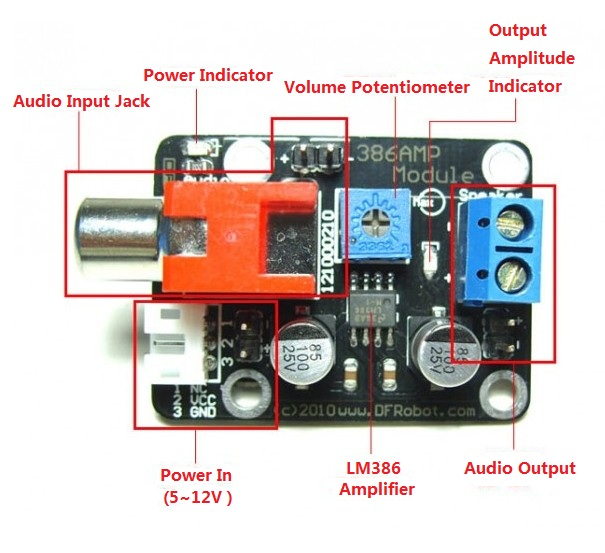
\includegraphics[scale=0.5]{386AMP.jpg}
\\
Cependant, il nous fallait un câble jack 3.5 vers RCA afin de pouvoir utiliser le module d'amplification sur lequel pouvait ensuite être aisément branché un haut-parleur. Étant donné que le laboratoire d'électronique ne possédait pas ce type de câble, nous avons fini par trouver le matériel nécessaire chez nous. Ainsi, nous avons pu faire les premiers tests du module avec nos téléphones. Ces derniers étant concluants, nous avons recherché les commandes nécessaires à la lecture d'un audio sur Raspeberry. Nous utilisons donc 3 fonctions systèmes
de la Raspeberry.
\begin{itemize}
    \item system("amixer -q set PCM,0 unmute"); permet de s'assurer que le son de la Raspeberry est actif
    \item system("mpg321 -q assets/" + filename + " \&"); permet de lancer, en processus d'arrière plan, l'audio désigné par la variable filename
    \item system("pkill -9 mpg321"); permet d'arrêtter le processus qui joue la musique en cours
\end{itemize}
Malheureusement, lors de notre premier test du module d'amplification sur la Raspeberry nous n'avons obtenu qu'un bip continu. Ce problème survient uniquement lorsque les autres fonctionnalités  de notre robot était en marche. Un autre groupe a été confronté à ce problème et malgré nos efforts communs et les nombreux cas similaires présents sur Internet nous n'avons jamais réussi à utiliser le module d'amplification.
\\
Les solutions que nous avons essayées sont pourtant nombreuses :
\begin{itemize}
    \item changement de configuration d'amixer (le logiciel gérant le son sur la Raspeberry)
    \item changement de matériel (module d'amplification et câble)
    \item changement de configuration du PWM (dont l'activation semble être à l'origine de notre problème)
\end{itemize}
En fin de compte, après l'échec de toutes ces solutions, c'est l'utilisation du MAX 98357A, un Amplifier/DAC (Digital Analog Converter), qui nous a permis de jouer des sons sur notre robot. Nous en avons donc conclu que le port jack de la Raspeberry était bien à l'origine de notre problème sans pour autant l'avoir résolu.

\subsection{Tentative d'algorithme suiveur de ligne PID}
Nous avons réalisé quelques recherches sur des algorithmes permettant de faire de l'asservissement et nous nous sommes rendus compte que l'algorithme le plus répendu est le PID Control.
L'objectif de cet algorithme est de faire en sorte que l'erreur entre la position actuelle du robot et la position désirée soit nulle. Pour cela, il faut calculer l'erreur, c'est à dire la différence entre la position actuelle et la position désirée, puis calculer la dérivée de cette erreur et enfin calculer l'intégrale de cette erreur.
Sur le papier, cet algorithme semble très simple à mettre en place. Cependant, nous avons rencontré de nombreuses difficultés lors de la mise en place de cet algorithme.
En effet, nous avons dû faire face à de nombreux problèmes de détection de ligne. En effet, nous avons essayé de faire fonctionner notre robot avec des capteurs QTR mais ces derniers ne fonctionnaient pas correctement. Nous avons donc essayé de faire fonctionner notre robot avec une caméra mais celles-ci n'avait pas un angle de vue assez large pour détecter la ligne suffisament loin pour le PID.

\subsection{Échec des capteurs QTR}
Nous avons essayé d'utiliser des capteurs QTR pour détecter la ligne. Cependant, nous avons rencontré de nombreux problèmes avec ces capteurs. En effet, nous n'avons rien trouvé sur internet qui nous permettait de les utiliser correctement avec un raspberry.
Nous avons donc développé notre propre code pour utiliser ces capteurs. Cependant, nous n'avons pas réussi à obtenir des résultats satisfaisants avec ces capteurs. En effet, ils détectaient trop de bruit et ne détectaient pas la ligne de manière fiable.
Nous ne savons pas si le problème venait de notre code ou des capteurs eux-mêmes mais nous avons finalement décidé de ne pas utiliser ces capteurs.
Nous nous sommes dit que le seul moyen de faire fonctionner notre robot correctement était d'utiliser une caméra. En effet, en observant une seule bande de pixel sur une image, nous pouvions détecter la ligne de manière fiable.


\section{Les capacités du robot}